\chapter{基于深度学习目标检测模型的云平台设计与实现}

基于深度学习的自动分拣系统,要实现大规模应用,需要深度学习目标检测模型的大规模应用。
基于国内制造业从业者普遍缺乏深度学习相关理论和应用知识的情况,本文设计的基于深度学习目标检测
模型的云平台可以帮助实现制造业的深度学习普及化。云平台的实现主要包括网页端设计和服务器端开发。
云平台主要用于存储接收用户自定义模型的超参数数据、训练深度学习目标检测模型。网页端则是云平台与
用户的交互工具,用于帮助用户自定义超参数,从而定制化所需的目标检测模型。

\section{深度学习云平台方案设计}

本文的深度学习云平台承担了训练深度学习模型的任务,这需要较强的计算能力。因此,本文的深度学习
云平台所用的后端服务器为2.2.2小节中的服务器。结合国内制造业的信息化现状,深度学习云平台的前端交互
方式为网页形式,该方式适用于PC端的Windows/macOS/Linux系统和手机端的浏览器,全方位覆盖,有利于
深度学习模型的普及化。

\subsection{云平台整体架构}

深度学习云平台可以分为四层:客户端层、传输层、服务器层和数据层。

1. 客户端层

客户端层即Web层,用于云平台与用户的交互。用户在网页上输入各种定制化参数,Web层负责收集用户输入的
参数,并将其封装发送出去。并且,Web层需要将模型训练过程中的参数实时展示出来。

2. 传输层

Web层与服务器层并非一对一的关系,而是多对一的关系,因此需要传输层将多个Web页面的数据传输到服务器层,并且
保证安全和高效。

该场景为经典的网络通信场景,因此可以使用TCP/IP通信协议,使用HTTP通信方式进行数据传输。

3. 服务器层

服务器层包括接收和处理客户端层发送来的数据和执行深度学习训练程序。接收数据同样使用传输层的方式,执行深度学习训练程序
则需要在后端程序中调用shell脚本,使用脚本来完成模型训练功能。同时,服务器层需要将训练过程中的参数实时传输到客户端层进行展示。

4. 数据层

数据层主要用来存储用户信息、用户定制化模型的参数以及模型训练日志。该层可以利用数据分析用户使用的模型参数,从而为用户推荐更加合适的参数。

\begin{figure}[htbp]
    \centering
    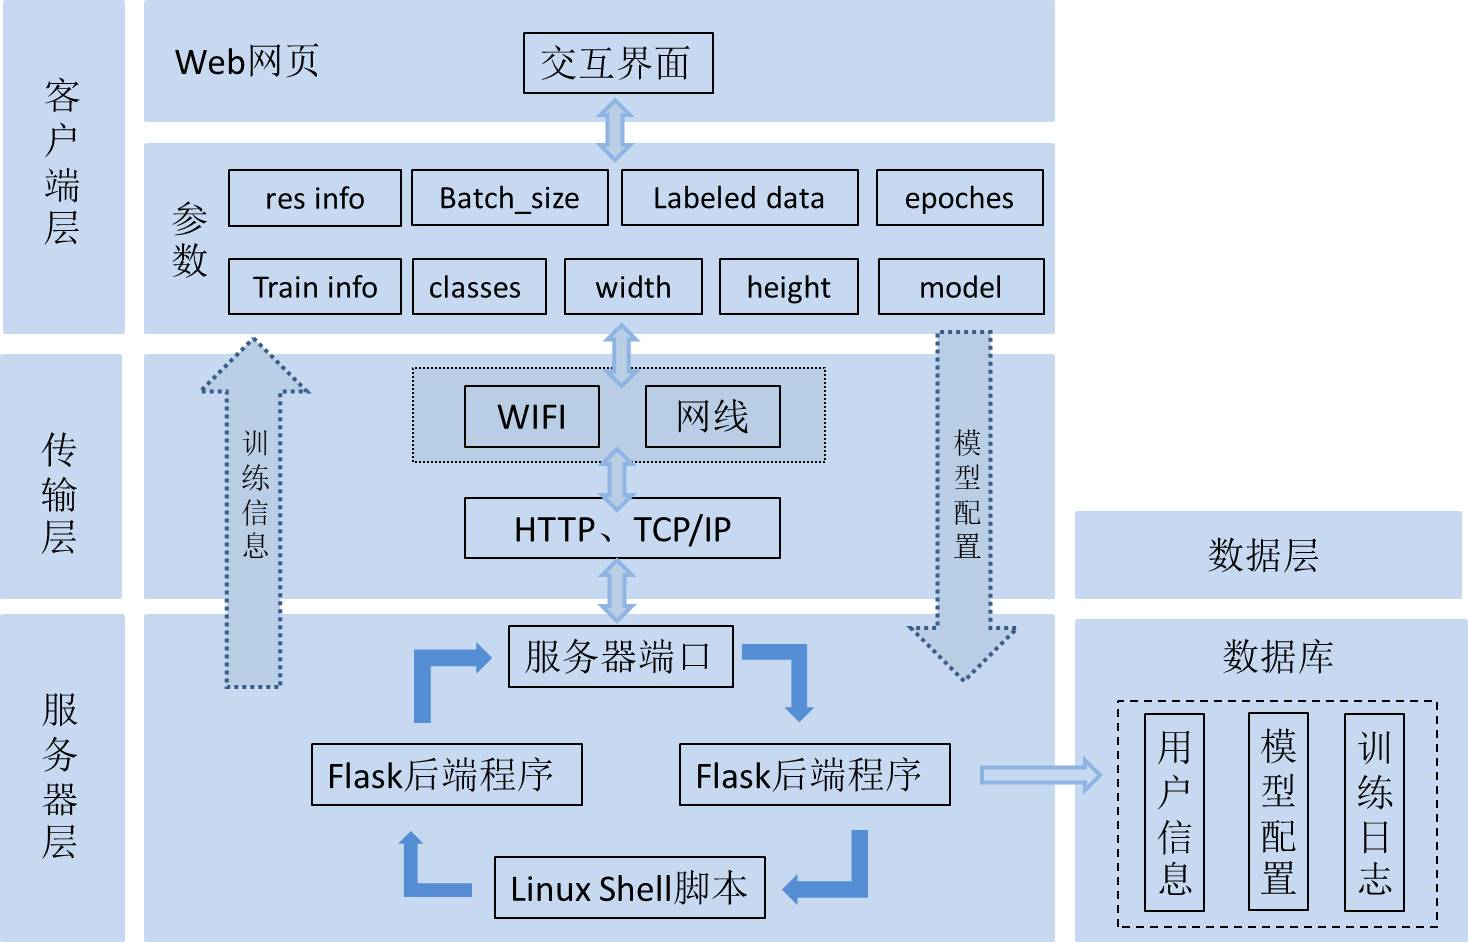
\includegraphics[width=\textwidth]{pic/chap4/cloudplatform_construct.jpg}
    \caption{基于深度学习目标检测模型的云平台总体架构}
    \label{fig:cloudplatform_construct}
\end{figure}
图 \ref{fig:cloudplatform_construct} 显示了云平台的总体架构。其中,客户端层的各项参数为客户端层与服务器层进行通信所需要的数据,
即传输层所需要传输的数据。各项参数的意义见表 \ref{table:Web:info}。

{
    \begin{table}[htb]
        \zihao{5}
        \caption{客户端层参数含义}
        \label{table:Web:info}
        \centering
        \begin{tabular}[t]{c|c|c|c|c|cc|c|c|c}
            \hline
            参数 & res info & Batch\_size & Labeled data & epoches & Train info \\
            \hline
            含义 & 服务器返回状态码 & 模型训练批次大小 & 标注数据集 & 模型训练轮次 & 模型训练信息\\
            \hline
            参数 & classes & width & height & model \\
            \hline
            含义 & 工件类别数 & 图片宽度 & 图片高度 & 选择使用的模型 \\
            \hline
        \end{tabular}
    \end{table}
}

\subsection{基于Http协议的通信方法分析}

本文设计的深度学习云平台主要用于制造业当中,目前国内制造业企业很少有自己的服务器,即私有云。与本地服务器进行局域网
通信的方案不具有普适性。因此,考虑使用公有云,即建立大规模服务器,集中维护与管理。企业只需使用客户端页面与公有云进行
交互,可以免去高昂的服务器购买、维护与管理成本。考虑到客户端的兼容性与分布式性质,客户端方案使用Web页面与用户进行交互。
即,用户使用浏览器访问云平台网页与服务器进行交互。

基于云平台为浏览器到服务器的应用模式,我们选择HTTP协议作为通信方式。HTTP \cite{HTTP} 是一种用于分布式、协作式和超媒体信息系统
的应用层协议。HTTP是万维网的数据通信的基础。基于HTTP协议,云平台客户端可以使用网线或WIFI或4G的通信手段,大大扩宽了
云平台的应用场景。

\subsection{云平台性能需求分析}

深度学习云平台承担着制造业深度学习模型普及的任务,为了保证良好的用户体验及云平台运行的稳定性,深度学习云平台的性能
需求如下:

1. 功能完整与稳定

云平台需要根据用户输入的个性化参数来实现模型训练。由于用户可能缺乏深度学习相关知识,因此云平台需要全面考虑所有
可能出现的情况并事先预定应对措施,如当用户没有给出参数时使用默认参数,用户输入非法或提供无用信息时给予正确提示。
总之,作为服务多个用户的云平台,其后台逻辑需要考虑周全,防止单个用户使用导致崩溃进而影响其他用户。

2. 可调试性

云平台作为前端、后端、脚本等一体化的复杂平台,需要建立完善的日志系统,方便在问题出现时进行调试,准确快速地定位问题所在,
进而快速排查,迅速回复运转状态。

3. 易用性

作为面向制造业从业者的深度学习云平台,云平台需要将深度学习相关知识深度封装,并在Web页面中对于每个可配置参数进行
引导与指示说明,并在Web页面中加入“Help”页面,对云平台的使用流程进行完整详尽的说明,帮助用户尽快上手云平台。

\section{基于Flask的Web服务端设计与实现}

Web页面收集用户定制化参数并将其打包发送到服务器固定端口,服务器端有程序不断地监视该端口并接收该端口信息。此
程序即为Web服务端程序。Flask是一个使用Python编写的轻量级Web应用框架。本文使用Flask \cite{Flask} 进行服务端程序的开发。

\subsection{云平台服务端架构}

服务器端需要部署一个后端程序,用于监控特定端口发送来的信息并给出响应。同时,该程序负责连接数据库,将用户信息、模型配置等
数据存放到数据库当中,并在需要时从数据库拿取数据;调用脚本程序,根据客户端发送来的配置更改Darknet配置文件,然后调用GPU训练深度
学习模型;将模型训练过程的各项参数与权重文件发送给客户端。

云平台服务端程序主要包括以下几个模块:

1. 主页面模块

当用户访问云平台网页端时,浏览器向服务端程序发送请求,服务端程序需要将主页面的HTML文件返回给客户端,将主页面展现给
用户。

2. 帮助中心模块

帮助中心模块负责给出对主页面的各项可配置参数的说明与指导,以及帮助刚接触云平台的用户熟悉使用流程。

3. 文件上传模块

文件上传模块负责接收用户在客户端上传的标注数据,并将其存放到特定文件夹,用于后续训练深度学习模型使用。

4. 数据库连接模块

数据库连接模块负责与数据库进行连接,将客户端传来的用户信息、模型配置等数据进行解析,然后存放到数据库中;同时在需要时
从数据库中拿取数据。

5. 模型训练模块

模型训练模块接收客户端传来的模型配置信息并进行解析,然后将配置信息封装为shell脚本的命令行参数,用来调用Darknet进行
深度学习模型训练。

其具体运行流程如图 \ref{fig:cloudplatform_process} 所示。

其中,每条“流程线”通过Flask后端程序的视图函数执行。Web浏览器(即客户端)将请求发送给Web服务器,Web服务器再把请求发送给
Flask程序实例。程序实例需要知道每个URL请求需要运行哪些代码,因此在Flask实例中保存有URL到Python函数的映射关系。处理URL和
函数关系的程序成为路由,这些函数称为视图函数。视图函数处理完成对应URL所需的代码之后,需要进行响应。由于本文使用的HTTP协议,
而HTTP协议需要的不仅是作为响应的字符串,还需要状态码,即表明请求处理结果状态的标识符。该标识符用于客户端控制显示的页面。Flask
后端程序启动之后,将运行日志进行保存管理,方便问题发生时进行问题定位和排查。

\begin{figure}
    \centering
    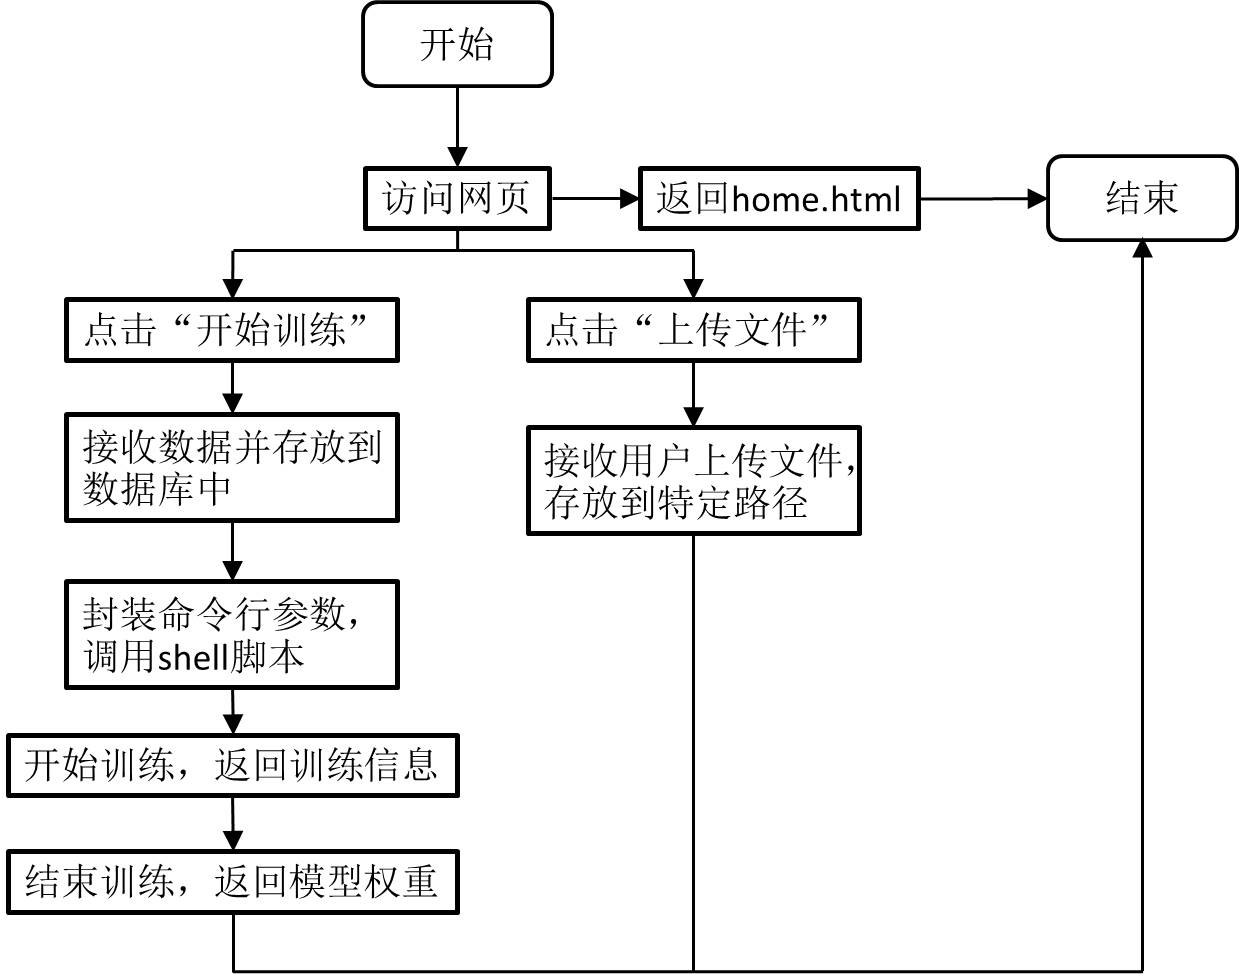
\includegraphics[width=\textwidth]{pic/chap4/cloudplatform_process.jpg}
    \caption{云平台运行流程图}
    \label{fig:cloudplatform_process}
\end{figure}

\subsection{云平台数据库设计}

基于深度学习的目标检测模型云平台的数据库包括用户信息数据和模型配置数据两类,两类数据分别存放于两个数据库表中,两个数据表
通过唯一主键进行关联映射。图 \ref{fig:database_table} 显示了两个表格之间的关系。其中用户id在用户第一次登录时在保证唯一性的前提下随机生成,用作
用户唯一标识和数据库表格主键。本文选用SQLite \cite{SQLite} 作为数据库,根据使用场景设计表格结构。

\begin{figure}
    \centering
    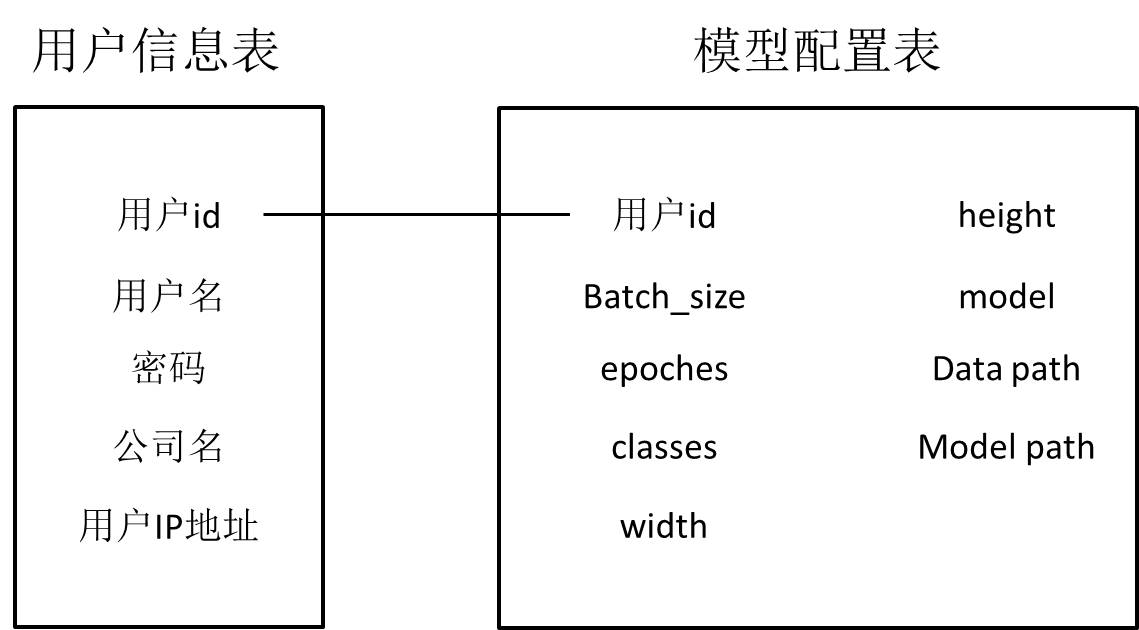
\includegraphics[width=\textwidth]{pic/chap4/database_table.jpg}
    \caption{云平台数据库表格关系示意图}
    \label{fig:database_table}
\end{figure}

其中,用户信息表各字段含义如表\ref{table:database:userInfo}所示。

用户信息表主要用来存放使用云平台的用户个人信息,便于进行用户管理和问题源定位。为了方便使用,云平台不设置注册和登录功能,用户名和密码用于
密匙,便于以后扩展云平台功能时将数据库相关数据对用户进行开放。云平台使用IP地址
对用户权限进行管理。因此,需要将用户IP地址存入表格。对用户的登录授权即开放其IP地址访问权限。当用户在浏览器输入域名时,服务端程序会将
其IP地址与已授权IP地址集合进行匹配,若其IP地址经过授权,则可正常使用。公司名称则用于管理和统计使用云平台的制造业企业。
此外,该表中的数据为用户第一次使用云平台时填写,单用户只需填写一次,
此后无需再次填写。

{
    \begin{table}[htb] 
        \zihao{5}
        \caption{模型配置表字段含义}
        \label{table:database:userInfo}
        \centering
        \begin{tabular}[t]{c|c|c|c|c|c|c}
            \hline
            编号 & 字段名称 & 字段含义 & 数据类型 & 必填字段 & 默认值 & 约束要求  \\
            \hline
            1 & user\_id & 用户唯一标识符 & Nvarchar & 是 & 无 & 主键\\
            \hline
            2 & username & 用户名 & Nvarchar & 是 & 无 & 无 \\
            \hline
            3 & passwd & 密码 & Nvarchar & 是 & 无 & 无\\
            \hline
            4 & company & 公司名称 & Nvarchar & 是 & 无 & 无\\
            \hline
            5 & ip & 用户ip地址 & Nvarchar & 是 & 无 & 无\\
            \hline
        \end{tabular}
    \end{table}
}

模型配置表各字段信息如表 \ref{table:database:modelInfo} 所示。

模型配置表大部分字段都由用户自定义完成,而data\_path字段,则是用户上传标注数据后产生的;model\_path字段为模型训练
完成后,产生的模型权重文件保存地址。用户每次使用云平台,该模型配置表都会新增一条数据。该表格中的数据可用于探索训练深度学习
模型的最优配置参数,从而在用户自定义模型时,为其推荐配置参数,提高用户体验和使用效果。

{
    \begin{table}[htb] 
        \zihao{5}
        \caption{模型配置表字段含义}
        \label{table:database:modelInfo}
        \centering
        \begin{tabular}[t]{c|c|c|c|c|c|c}
            \hline
            编号 & 字段名称 & 字段含义 & 数据类型 & 必填字段 & 默认值 & 约束要求  \\
            \hline
            1 & user\_id & 用户唯一标识符 & Nvarchar & 是 & 无 & 主键\\
            \hline
            2 & batch\_size & 模型训练批次大小 & Int & 是 & 16 & 无 \\
            \hline
            3 & epoches & 模型训练轮次 & Int & 是 & 2000 & 无\\
            \hline
            4 & classes & 工件类别数 & Int & 是 & 无 & 无\\
            \hline
            5 & width & 图片宽度 & Int & 是 & 无 & 无\\
            \hline
            6 & height & 图片高度 & Int & 是 & 无 & 无 \\
            \hline
            7 & model & 选择使用的模型 & Nvachar & 是 & Yolov3 & 无 \\
            \hline
            8 & data\_path & 用户标注数据路径 & Nvachar & 是 & /data/cloud/data/ & 无 \\
            \hline
            9 & model\_path & 模型权重文件路径 & Nvachar & 是 & /data/cloud/model/ & 无 \\
            \hline
        \end{tabular}
    \end{table}
}

\subsection{基于Linux的Shell脚本实现云平台模型训练}

云平台的模型训练模块需要进行数据预处理、更改模型配置文件、调用Darknet进行模型训练等操作,这一系列操作无法在Flask后端程序
中单独完成,因此,考虑编写Linux的Shell脚本 \cite{Shell} 来完成以上工作,在Flask后端程序中只需构造命令行参数和执行shell脚本,即可完成
以上所有步骤。

具体来说,Shell脚本需要完成以下任务:

1. 解压文件

用户上传的标注数据集为压缩格式,Shell脚本需要判断压缩数据的具体格式,如rar、tar.gz等,根据具体格式选择压缩
工具进行解压,将jpg和txt格式的图片和标注文件保存到特定目录下,用作后续处理。

2. 训练集测试集划分

用户上传的标注数据需要随机打乱后,划分为训练集测试集。默认训练集占90\%,测试集占10\%。训练集用作训练模型,
测试集用于验证最佳权重参数,验证模型效果。这一步可以使用Shell脚本实现,也可以用Python实现后,在Shell脚本中
执行Python脚本,本文使用后者实现。这一步最终的结果是将训练集和测试集的文件路径分别保存到特定的文件中。

3. 模型文件配置

Shell脚本需要根据用户自定义的模型配置更改Darknet中的模型配置文件。这一步需要读入命令行参数,然后使用sed命令
替换Darknet中模型配置文件需要更改的配置,产生用于训练用户定制化模型的配置文件,以便后续模型的训练。

4. 模型训练

这一步,Shell脚本需要切换目录到Darknet主文件夹,调用命令进行训练。同时,Shell脚本需要实时监控训练信息,并将
主要的训练信息读取并发送到Flask后端程序,以提供给客户端。另外,模型训练结束后,Shell脚本需要将模型文件最终保存路径
记录并发送给Flask后端程序,以供客户端下载。

\section{基于Web前端的客户端系统设计}

Web前端承担着与制造业企业用户交互的责任,是服务器端深度学习模型训练的深度封装。Web端的优势是简单易用,覆盖设备广泛,
能够快速与云平台进行交互,有效降低深度学习模型训练和应用的门槛。

\subsection{客户端网页需求分析}

Web前端页面主要需求如下:

(1) 主页面设计,要求美观简洁,交互方便。

(2) 实现下拉框和文本框设计,用于用户自定义模型配置。

(3) 实现用户文件上传功能,包括用户上传文件后缀名合法性检测,文件上传进度展示,文件上传成功提示。

(4) “开始训练”按钮的实现,及触发函数绑定。触发函数需要实现下拉框和文本框数据收集和封装,并发送HTTP请求给服务器端。

(5) 服务器端模型实时训练信息的接收,并将训练信息实时展示到Web页面前端。该项信息需要在“开始训练”按钮按下之后进行展示。

(6) 服务器端模型权重文件的下载。模型训练完毕之后,Web前端页面需要展示“下载模型”按钮,用户点击之后可以下载训练完成的深度学习
目标检测模型权重文件,该权重文件可直接应用于工件的目标检测。

\subsection{客户端页面设计与实现}

云平台网页界面主要有两个网页组成,Home界面和Help界面。各个界面功能如表 \ref{table:Web:features} 所示。

{
    \begin{table}[htb] 
        \zihao{5}
        \caption{云平台网页各页面功能介绍}
        \label{table:Web:features}
        \centering
        \begin{tabular}[t]{c|l}
            \hline
            界面名称 & 界面介绍   \\
            \hline
            Home & 1. 标注数据上传 \\
             & 2. 模型超参数配置 \\
             & 3. 模型训练信息展示 \\
             & 4. 模型权重文件下载 \\
            \hline
            Help & 云平台使用文档 \\
            \hline
        \end{tabular}
    \end{table}
}

本文使用HTML、CSS、Javascript \cite{JS} 技术进行上述界面的开发。其中,HTML用来编写网站页面UI;CSS用于定制UI特性;JavaScript用于
UI各组件的逻辑处理与网络收发。即HTML负责网页的内容,CSS负责网页的样式,Javascript负责网页的逻辑。

网页设计的准确思路将网页分成三个层次:结构层(HTML)、表示层(CSS)、行为层(Javascript)。这种分层次的网页设计思路
将网页的各项内容、样式和逻辑分开处理,便于组织和管理代码,使得程序更加直观,更加易于调试。Web前端的整体架构如图\ref{fig:web_construct}
所示。

\begin{figure}[h]
    \centering
    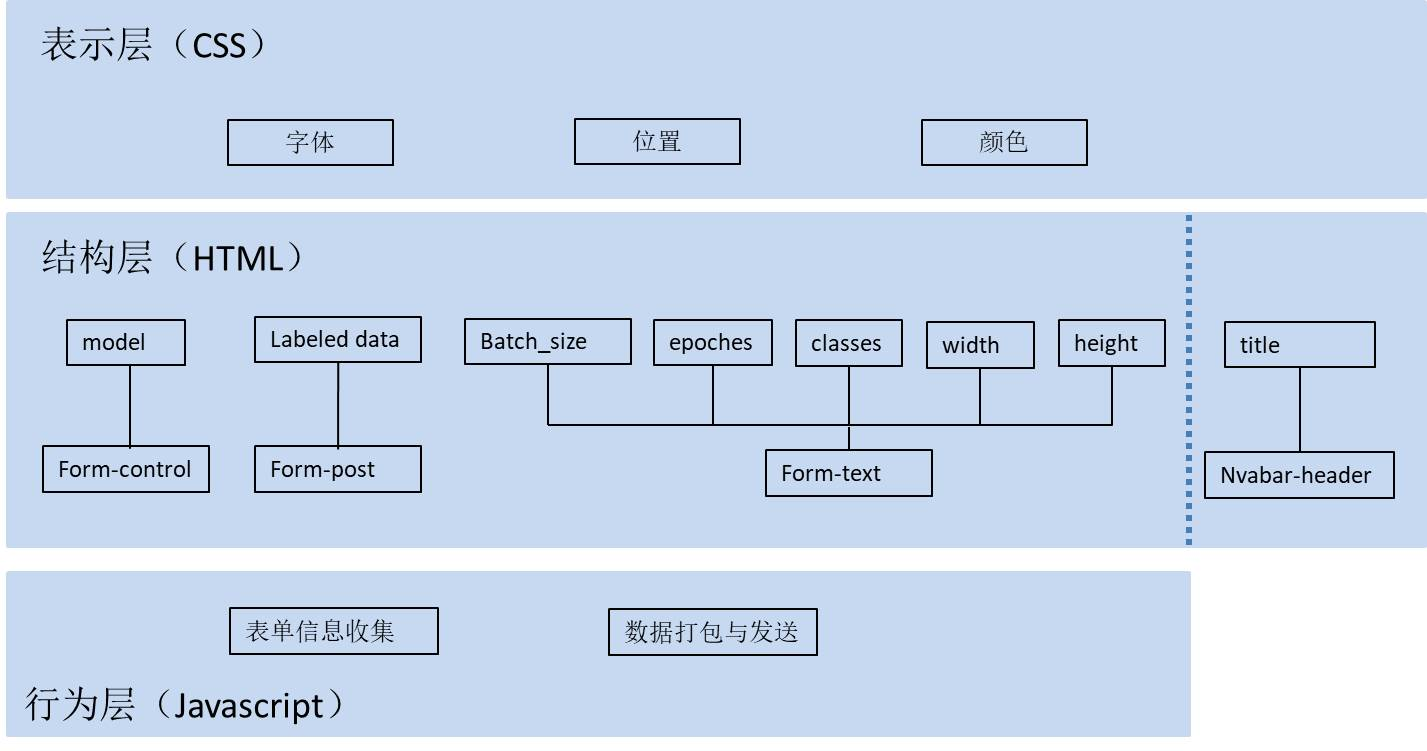
\includegraphics[width=\textwidth]{pic/chap4/web_construce.jpg}
    \caption{云平台Web前端结构图}
    \label{fig:web_construct}
\end{figure}

其中,网页所展示的所有内容和其层次结构由结构层产生;网页内容的字体、颜色、位置和样式由表示层组织;网页所要实现的功能及其
和服务器端所实现的各种交互由行为层负责。

为了简洁与便于管理,本文的Web页面使用了Bootstrap \cite{bootstrap}前端框架进行开发。Bootstrap是一个用于快速
开发Web应用程序和网站的前端框架,基于HTML、CSS和JavaScript实现。同时,Bootstrap支持市面上几乎所有
的浏览器,符合云平台的定位。

使用Bootstrap设计开发Web前端页面各组件的方法如下:

1. 顶部导航栏

Bootstrap中预置了Twitter风格的导航栏,在home.html中需要导入bootstrap/base.html,然后根据可根据模板设计出对应的导航栏。本文设计
的云平台导航栏分别链接到Home和Help页面。效果如图 \ref{fig:topbar_ui} 所示。

2. 模型选择下拉框

使用下拉选择框的场景为用户选择使用的模型。下拉选择框使用HTML表单实现,HTML表单用于收集用户输入。下拉框属于表单的一种,用于选择信息。其HTML标签为<form-group>,二级标签为<option>,
下拉选择框共三个选项,供用户选择需要训练的深度学习模型,给出的选择项为Yolov1,Yolov2和Yolov3,默认为Yolov3。实现效果如图 \ref{fig:model_ui} 所示。

3. 文本输入框

文本输入框用于用户输入识别物体类别数、训练模型的Batch\_size、训练模型的轮次、图片高度和图片宽度。文本输入框同样使用HTML表单实现。其HTML
标签为<form>,二级标签为<input>。与下拉选择框用户只能在有限的选项中进行选择不同,文本输入框赋予了用户输入任何可能字符的能力,但表单需要的信息
是有格式要求的,如物体类别数需要为整型。因此,对于文本输入框,在JavaScript的逻辑处理中需要进行合法性判断。当不合法时,该框将给出提示。文本输入
框的实现效果如图 \ref{fig:input_ui} 所示。
 
4. 文件上传模块

文件上传模块相对特殊。文件上传模块需要和服务器进行直接交互,而非通过JavaScript进行交互。由于云平台Home页面是通过HTTP的GET方法获取,因此考虑使用POST方法进行文件
上传。服务器端视图函数进行判断,若客户端发送的为GET请求,则返回home.html,若为POST请求,说明为文件上传模块发送的请求,视图函数通过程序上下文接收Web表单,解析
表单数据获取文件,并将文件保存到特定路径。文件上传模块的HTML标签为<form>,标签对应方法(method)为post。实现效果如图 \ref{fig:upload_ui} 所示。

5. 开始训练按钮

开始训练按钮使用正常的HTML标签生成,其标签为<button>。需要注意的是,该按钮绑定了JavaScript代码,用于处理Web的整体逻辑。因此在按钮的HTML标签中需要加入监听
函数onclick="startTrain()",该函数监听按钮状态。当按钮被按下是,JavaScript的监听函数被触发,从而执行相关逻辑。

6. Help页面

Help页面主要为帮助文档,使用Markdown编写后生成html代码即可。

\begin{figure}[h]
    \begin{minipage}[t]{0.45\textwidth}
        \centering
        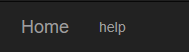
\includegraphics{pic/chap4/topbar_ui.png}
        \caption{导航栏UI效果}
        \label{fig:topbar_ui}
    \end{minipage}
    \begin{minipage}[t]{0.45\textwidth}
        \centering
        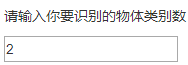
\includegraphics{pic/chap4/input_ui.png}
        \caption{文本输入框UI效果}
        \label{fig:input_ui}
    \end{minipage}
\end{figure}

\begin{figure}[h]
    \begin{minipage}[t]{0.45\textwidth}
        \centering
        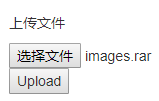
\includegraphics{pic/chap4/upload_ui.png}
        \caption{文件上传UI效果}
        \label{fig:upload_ui}
    \end{minipage}
    \begin{minipage}[t]{0.45\textwidth}
        \centering
        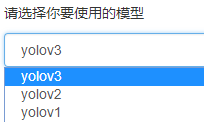
\includegraphics{pic/chap4/model_ui.png}
        \caption{下拉框UI效果}
        \label{fig:model_ui}
    \end{minipage}
\end{figure}

网页整体UI如图 \ref{fig:total_ui} 所示。

\begin{figure}[h]
    \centering
    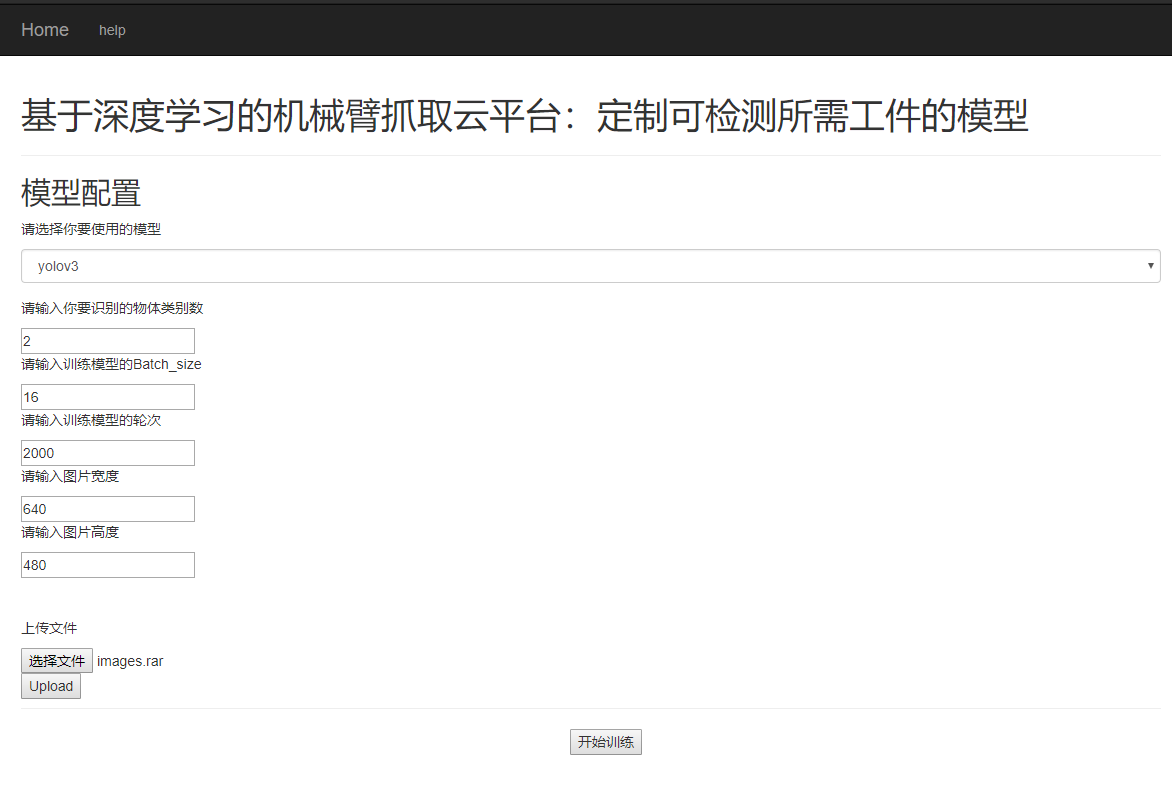
\includegraphics[width=0.9\textwidth]{pic/chap4/total_ui.png}
    \caption{Web页面整体UI效果}
    \label{fig:total_ui}
\end{figure}

网页的行为层代码采用JavaScript代码,主要实现前端页面“开始训练”按钮的行为逻辑。即该按钮的监听函数startTrain()。该函数需要实现的功能及实现方法如下:

(1)获取下拉选择框和文本输入框信息,并使用JavaScript变量进行引用。JavaScript可以使用document.getElementById方法获取HTML中的表单信息,该方法的输入
为HTML中各个组件事先定义的唯一id。下拉选择框信息的获取则需要先获取选择项数组和当前选择项的索引值,然后再获取当前选项值。

(2)判断文本输入框输入的合法性。若输入非法,需要提示用户修改输入,直到所有输入合法为止。云平台要求使用文本输入框输入的模型超参数均为Int整型,因此需要对
步骤一中获取的文本输入框信息变量进行类型判断,若不合法,则使用alert()函数进行网页弹窗,提醒用户输入出错,要求重新输入。

(3)将各项信息封装为JSON\cite{JSON}格式,用于后续传输。JSON将各项参数保存为键值对的形式,由花括号进行封装,数据由逗号分隔。
JSON层次简洁清晰,易于人阅读和编写,同时也易于机器解析和生成,能够有效提高编码和网络传输效率,非常适用于云平台传递各项参数的
应用场景。JavaScript中可使用JSON.stringify()方法进行JSON数据封装。

(4)向服务器发送HTTP POST请求,将封装好的数据发送到服务器,同时接受服务器返回的信息,根据返回信息作出相关判断。若上传成功,则在用户
前端进行相应提示,否则给出错误提示。JavaScript使用XMLHttpRequest()方法开启HTTP数据传输通道,调用onreadystatechange()回调函数可监听
服务器状态码,使用send()方法将步骤(3)中封装好的数据发送到服务器。

\section{本章小结}

本章首先介绍了基于深度学习的目标检测模型云平台的整体架构,云平台主要由服务器端和Web前端组成。之后本章分别
介绍了服务器端和Web前端的设计架构和实现方法。


